
\documentclass[conference]{IEEEtran}
\usepackage[utf8]{inputenc}
\usepackage[T1]{fontenc}
\usepackage[UKenglish]{babel}
\usepackage{cite}
\usepackage{graphicx}
\usepackage{subfig}
\usepackage{todonotes}
\usepackage[cmex10]{amsmath}
\usepackage{hyperref}
%\parskip 2ex % TODO Remove
\usepackage{dblfloatfix}
\usepackage{xfrac}

\begin{document}
\title{Energy-efficient Routing Protocols for Mobile ad-hoc Networks}
\author{\IEEEauthorblockN{Julian Andres Klode}
\IEEEauthorblockA{Philips-Universität Marburg \\
Email:\href{mailto:klode@mathematik.uni-marburg.de}{klode@mathematik.uni-marburg.de}}}

\maketitle


\begin{abstract}
Mobile Ad-Hoc networks, with battery-powered nodes, require energy efficient
routing protocols in order to reduce the power consumption of nodes. We will
take a look at which categories of energy-efficient routing protocols exist,
and show examples for each category.
\end{abstract}


\section{Introduction}
Mobile ad-hoc networks present a number of unique challenges for routing protocols.
Their nodes are battery-powered and non-stationary, requiring flexible network architecture.
One example for ad-hoc networks, albeit not particularly mobile, are wireless sensor networks.

Routing protocols in such networks need to consider several important key
factors:
\begin{enumerate}
   \item Scalability -- A protocol should scale to a large number of nodes
   \item Fault tolerance -- A protocol should continue working if some nodes fail
   \item Energy efficiency -- A protocol should not consume more energy than needed,
   either on an individual node, or aggregated.
\end{enumerate}

A recent survey\cite{alotaibi2012survey} on routing protocols for wireless
ad hoc networks describes six categories of routing protocols for wireless
ad-hoc networks,  in addition to the classic categories of proactive (that is, table driven)
and reactive (that is, on demand) routing protocols:
\begin{enumerate}
  \item Geographical
  \item Geo-cast
  \item Multi-Path
  \item Hierarchical
  \item Power-aware
  \item Flow-Oriented
  \item Hybrid
  \item WMN
  \item Multicast
\end{enumerate}

Most of these categories are not focused on energy efficiency, but more on
other factors such as fault tolerance, scalability and performance. The only
category in which energy efficiency is discussed is that of power-aware algorithms.


\section{Categories of ad-hoc routing protocols}
Classic routing protocols are categorised in two dimensions:
centralized/distributable and proactive/reactive.
The unique challenges inherent in wireless ad-hoc networks led to a larger
amount of categories, which are not always necessarily disjoint, meaning
that an algorithm may belong to one or more categories.

\subsection{Basics: Proactive routing}
In proactive routing algorithms, each router builds its routing table by
(regularly) exchanging messages with other routers in the network.

This has the advantage that routing information is already available when a
package is to be routed.
A huge disadvantage of proactive routing protocols is the overhead imposed
by the exchange of the update messages.

\subsection{Basics: Reactive routing}
In a reactive routing algorithm, routes are discovered when a packet arrives
from a source and needs to be delivered to some destination.
While the routes need to be discovered more often than in proactive algorithms,
there is no traffic overhead due to the lack of special control messages, and
as such, the reactive approach is considered to scale better.

\subsection{Geographical routing}
The basic idea behind geographical routing is that nodes are addressed by
their geographic location instead of an IP address. This has the advantage
that each node does not need to know the full network topology, but each
node needs to know its location and each source needs to know the location
of the receiver.

We will take a look at the GAF protocol, which utilises geographical
features for routing, although with an interesting twist.

\subsection{Geo-cast}
Geo-cast routing merges multi-cast routing with geographical routing, to
deliver messages to a group of nodes identified by their locations.

\subsection{Hierarchical RA}
A hierarchical routing algorithm defines multiple zones or clusters with
gateways that connect them with each other. Inside a cluster, there often
are one or more cluster heads, that are responsible for maintaining the
connectivity within the cluster. Non-head nodes can only communicate with
their cluster heads, whereas gateway nodes can exchange information with
other clusters.


\subsection{Multi-path}
In a multi-path routing algorithms, multiple paths exists from one source
to a destination. The obvious advantages of a multi-path routing
algorithm include fault tolerance (if one path fails, another is still in
use), load distribution (congested routes can be avoided by chosing alternative
routes), peak performance (multiple routes may be used in parallel for different
parts of data).

Energy-efficiency is not a paramount concern of most multi-path routing, the
load balancing idea can however not only be applied to performance, but also
to power levels, to distribute the power used within the network, as we will
see later on. Such an algorithm would of course also be power-aware.

\subsection{Power-aware}
A power-aware routing algorithm tries to find a good trade off between
power consumption of nodes and mobility. \cite{main1} describes two categories
of power-aware protocols: those that try to minimise the active communication energy -- either
by controlling the power used for transmission, or by load control -- and
algorithms that try to minimise the inactivity energy, for example, by putting
rarely used nodes to sleep.

\subsection{Hybrid}
A hybrid protocol starts off as a proactive routing protocol but switches
to reactive routing for newly added nodes in order to reduce the control
overhead of proactive routing. In ad-hoc networks, it is implemented in
hierarchical network architectures.

\subsection{Flow-oriented}
\todo[inline]{Describe flow-oriented routing}
\subsection{WMN}
\todo[inline]{Describe WMN routing}
\subsection{Multicast}
\todo[inline]{Describe multicast routing}

\section{Survey of energy-efficient protocols}
\subsection{Transmission power control}
Protocols in this category try to minimise the power required to transmit
a message.
\todo[inline]{Give overview of strategies}

\subsubsection{Flow argumentation routing (FAR)}
Flow argumentation routing (FAR) was discussed by Chang and Tassiulas\cite{chang2000energy};
\todo[inline]{Describe FAR}
\subsubsection{Online max-min (OMM)}
\begin{figure*}
\centering
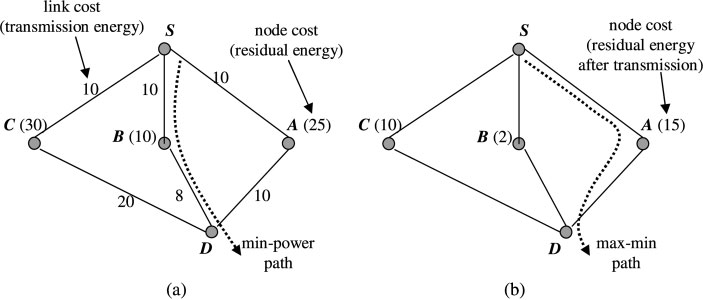
\includegraphics[width=0.7\textwidth]{images/omm}
\caption{Paths in OMM (from \cite{alotaibi2012survey})}
\label{ommex}
\end{figure*}

OMM \cite{li2001online} maximises the network lifetime using two metrics:
\begin{enumerate}
  \item \textbf{min-power} - Minimising the overall power
  \item \textbf{max-min} - Maximising the minimum residual power
\end{enumerate}

First OMM calculates the \textit{min-power} path using Dijkstra’s algorithm. Let
the power required by that be $P_{min}$.
Then it determines the \textit{max-min} paths by looking at all paths whose
power do not deviate much from the min-power path, that is, less than $zP_{\min}$
for some $z \ge 1$. It calculates the minimum residual power of all nodes
after the transmission would have taken place, and chooses the path where
that value is largest.

For example, in figure~\ref{ommex}, we can see that the min-power path from
$S$ to $D$ is $S \to B \to D$ with a value of 18 ($S \to A \to D$ has 20,
$S \to C \to D$ has 30).
It's minimum residual energy will be $2$, as node $B$ needs
$8$ out of the $10$ power units it has.

Looking at the alternate paths, we see that $S \to C \to D$ will have a
minimum residual energy of $30-20=10$ in node $C$, and $S \to A \to D$ will
have a minimum residual energy of $25-10$ in node $A$.
Thus, the max-min path is $S \to A \to D$.

Choosing a good value for $z$ in $zP_{\min}$ is important: For $z=1$, only
the min-power path is considered; for $z \to \inf$, all paths can be
considered. The algorithm starts with a \textit{random} value for $z$, and
then measures the residual energy (\textit{lifetime}) of of the most overloaded node during some
fixed time period. Afterwards, the value of $z$ is increased by a small constant
and the lifetime is measured again. If the lifetime increases, the value of $z$
is increased, otherwise, it is decreased. Because the lifetime is measured
in two distinct time periods, it is assumed that load distribution is roughly
similar, otherwise the results might not be really useful.

\subsubsection{Power aware localized routing (PLR)}
PLR\cite{stojmenovic2001power} is a geographical routing protocol, at least
to a certain extend, that tries to minimise the overall power usage. Each node
selects the next hop based on the power required for sending to this node, and
sending from that node indirectly to the destination.

For this, it has to know the locations of the next hops and the location of
the destinations. Based on the locations and the distance between the locations,
it can then estimate the power usage.

For direct connections, this is:
\( p(d) := ad^{\alpha} + c \)
for some constants $a$ and $c$ and some $\alpha > 2$ (that is, power usage
is at least growing quadratic in relation to the distance).

For indirect communication between the next hop and the final destination,
the power usage can be calculated as:
\begin{align*}
   q(d) &:= cn + da \left(\sfrac{a(\alpha - 1)}{c}\right)^{\sfrac{(1-\alpha)}{\alpha}}, \\
      n &:= d\left(\sfrac{(a(\alpha - 1))}{c}\right)^{\sfrac{1}{\alpha}};
\end{align*}
where $n-1$ is the optimal number of intermediate nodes\cite{stojmenovic2001power}.

So, given an example like figure~\ref{plrexample} with a source node $A$, neighbours $N_{1}$, $N_{2}$, and $N_{3}$, and a
destination $D$, $A$ should chose the next hop as the $N_{i}$ for which
$p(|AN_{i}|) + q(|N_{i}D|)$ is minimal.

\begin{figure*}
\centering
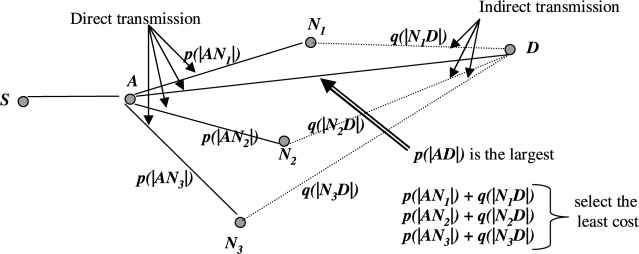
\includegraphics[width=0.7\textwidth]{images/plr-example}
\caption{Selection of next hop in PLR (from \cite{alotaibi2012survey})}
\label{plrexample}
\end{figure*}

\subsubsection{Minimum energy routing (MER)}
MER\cite{doshi2002demand} modifies the dynamic-source-routing (DSR)\cite{johnson1996dynamic}
and 802.11 MAC algorithms\cite{woesner1998power} with 8 options\ref{tbl:mer-options} in order to
(1) obtain power information, (2) measure overhead of energy-awareness, and
(3) maintain the minimum power route with mobile nodes.

\begin{table}[tb]
  \begin{tabular}{ll}
    Options & Implementation Level  \\
    \hline
    A: Routing packet-based power control & Routing software/\\ &802.11 firmware \\
    B: Minimum energy routing & Routing software \\
    C: Cache replies off & Routing software \\
    D: Internal cache options & Routing software \\
    E: Multi-hop route discovery & Routing software \\
    F: MAC layer ACK power control & 802.11 firmware \\
    G: Route Maintenance with power sensing & Routing software \\
    G: HMAC-Level snooping and gratious replies & 802.11 firmware \\
  \end{tabular}
  \caption{Options in MER}
  \label{tbl:mer-options}
\end{table}

Option $A$ modifies \textit{route-request} packages of the DSR protocol to
include the power used by the sender, which can the be added to the power
of the receiver to calculate the minimum power required for transmissions
from that sender to it. The value is appended at each intermediate node, and the
destination node then includes it in its \textit{route-reply} header.

The source node than includes this information when it's sending a packet, and
all nodes transmit that package with the controlled power level.

Option F does the same for the MAC layer's ACK packets.

Option $B$ is related to the route cache of the DSR protocol ($C$ and $D$ as well). It
uses the information obtained by option $A$ to select the route that requires
the minimum energy amongst its cached routes.

Option $G$ takes care of adjusting routes when the power transmittion requirements
change because nodes moved.

Option $E$ and $H$ allow nodes not participating in the routing to recommend
alternative, more energy-efficient, routes.

\subsubsection{Retransmission-energy aware routing (RAR)}
Discussed by Banarjee and Misra \cite{banerjee2002minimum};
\todo[inline]{Describe RAR}
\subsubsection{Smallest common power (COMPOW)}
Discussed by Narayanaswamy, Kawadia, Sreenivas and Kumar\cite{narayanaswamy2002power};
\todo[inline]{Describe COMPOW}

\subsubsection{PARO}
The PARO Protocol\cite{gomez2003paro} introduces intermediate nodes into a
route, increasing the length of the route, in order to reduce the transmission
power required by each node.

\subsection{Load distribution}
Power-aware load distribution (or `control') algorithms distribute the the
traffic based on the energy levels of the routers.
They do not try as much as the other algorithms to minimise the power required,
but instead focus more on distributing the power requirements among the available (routing) nodes.

\subsubsection{Local Energy Aware Routing Protocol (LEAR)}
Woo et al. introduced LEAR\cite{woo2001non},
\todo[inline]{Describe LEAR}

\subsubsection{Conditional max-min battery capacity routing (CMMBCR)}
Too introduced CMMBCR\cite{toh2001maximum}.
\todo[inline]{Describe CMMBCR}

\subsubsection{Dynamic Source Routing Power-Aware (DSRPA)}
In DSRPA\cite{djenouri2006dynamic}, nodes with the freshest battery are
chosen to route the packages, in order to achieve connectivity for as
long as possible.\cite{alotaibi2012survey}
\todo[inline]{Expand on DSRPA}

\subsubsection{Infra-Structure AODV for Infrastructured Ad-Hoc networks (ISAIAH)}
ISAIAH\cite{lindgren2002infrastructured} is an ad-hoc distance vector routing
algorithm. It routes similar to AODV, but selects routes that pass through
so called power base station (PBS) instead of mobile nodes, in order to reduce
the power consumption of the mobile nodes.

As with PARO, the routes chosen by this algorithm are longer than needed, but
because more nodes are stationary, the power consumption on the mobile nodes
is reduced.

\subsection{Sleep/power­ down mode}
Algorithms in this category try to minimise the time a node is active, and
maximise the time a node is at sleep. A common apprach to do this is to select
one or more masters from a set of nodes which take over the routing functionality
while the others can safely sleep. In such a scheme, nodes periodically wake up
and elect a new master if the current one goes away.

We will take a look at three master slaves protocols: SPAN, GAF, and PAMA;
and at one protocol called PEN that has no concept of master and slave nodes.

\subsubsection{SPAN}
\begin{figure*}
\centering
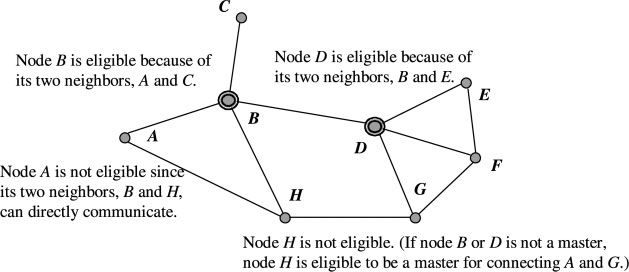
\includegraphics[width=0.8\textwidth]{images/span-master-example}
\caption{Master eligibility rule in the SPAN protocol. (from \cite{alotaibi2012survey})}
\label{spanmaster}
\end{figure*}
In Span\cite{chen2002span}, a master is selected based on the following rule:
A node becomes a master if two of its neighbors cannot reach each other directly
or via one or two masters. For example, in figure~\ref{spanmaster}, nodes B and
D become masters.

In order to prevent or reduce overloading of masters, masters periodically
check whether they should withdraw from being master; and non-master nodes
periodically check if they should become master.


\subsubsection{Geographic adaptive fidelity (GAF)}
\begin{figure*}[!t]
\subfloat[Grid example]{%
  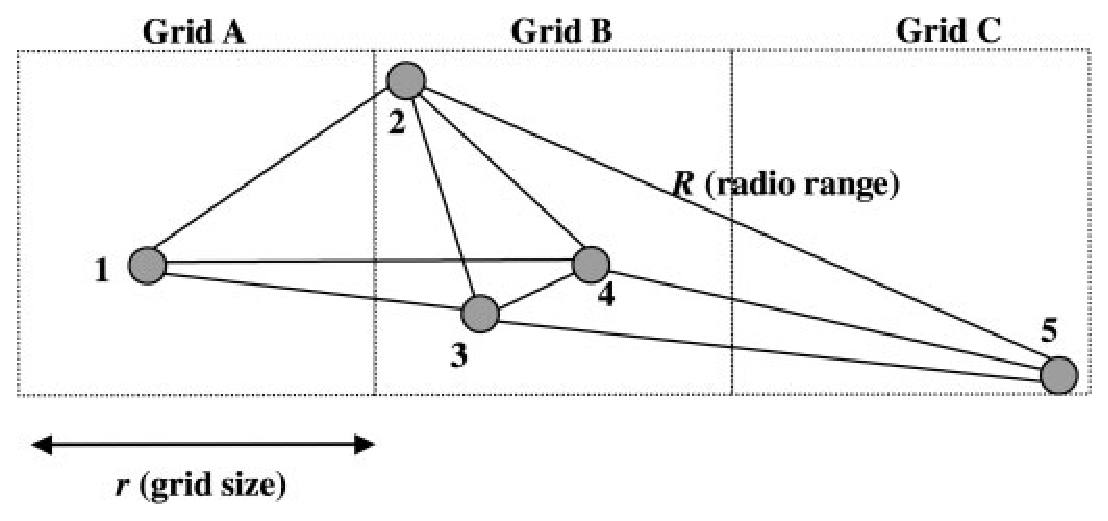
\includegraphics[width=0.46\textwidth]{images/gaf-grids}
  \label{gafgrids}
}
\hfill
\subfloat[Node states]{%
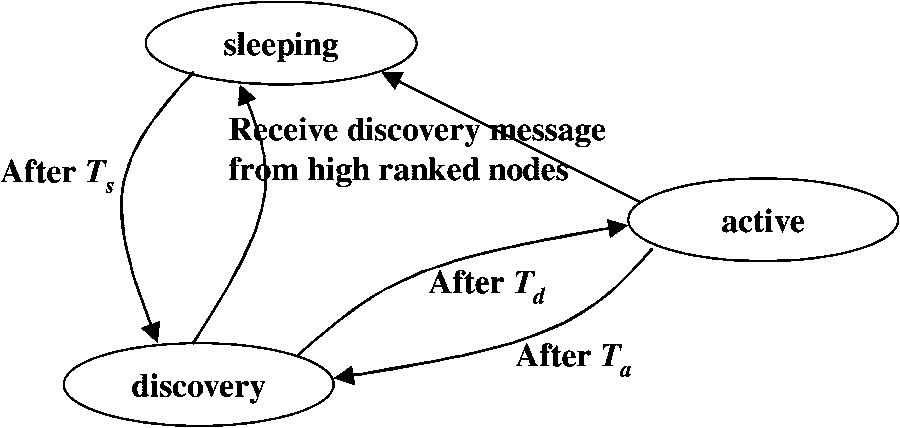
\includegraphics[width=0.46\textwidth]{images/gaf-states}
\label{gafstates}
}
\caption{Example grid and state diagram for GAF from \cite{alotaibi2012survey}}
\end{figure*}
GAF\cite{xu2001geography} uses the geographical (GPS) location of a node in
order to position them into a virtual grid.

Within each grid, the node with the highest residual energy becomes the master
of the grid, responsible for routing messages through that grid, while the
slave nodes can be put to sleep and will alternate between sleep and listening
states. For example, in grid B of figure~\ref{gafgrids}, one of 2,3,4 can be the
master of grid B and forward messages between A and B, while the other two can
be put to sleep.

Nodes have three states, as shown in figure~\ref{gafstates}: active for some time span $T_{a}$, in which they
act as the master of the grid; discovery for some time span $T_{d}$, in which a
master is elected - a node becomes the master if it hears no more discover messages
for time span $T_{d}$; and finally, a node can be sleeping.




\subsubsection{Power-Aware Multi-Access Protocol with Signaling Ad-Hoc Networks (PAMAS)}
PAMA\cite{singh1998pamas} controls the power usage based on the activity of
a node: Nodes that are not involved in the transmission of packages are turned
off for some time, without even affecting the delay or throughput of the
protcol.\cite{singh1998pamas} \todo[inline]{IS PAMA master-slave?}

\todo[inline]{More details on PAMA}

\subsubsection{Prototype embedded network (PEN)}
PEN\cite{girling2000design} does not follow the usual master-slave scheme
used by the other protocols. Nodes periodically wake up, advertise their
by broadcast messages, and then listen for any communication requests before
powering down again.

A sending node waits until it receives a broadcast message from the intended
destination, then sends a communication request to the destination during
the destinations listening period. Finally, it starts the communication.

This scheme easily avoids the cost of selecting a master and of overloaded
masters. It is only effective for networks without much traffic, as the delay
can be quite high because senders need to wait for receivers to wake up.



\subsection{Uncategorised}

\subsubsection{Energy Saving Dynamic Resource Routing Protocol (ESDSR)}
ESDSR\cite{tarique2005energy} \ldots{}

\todo[inline]{Categorize and describe ESDSR}
\subsubsection{Local Minimum Energy Dynamic Source Routing Protocol (MEDSR)}
MEDSR\cite{tanque2007minimum} \ldots{}
\todo[inline]{Categorize and describe MEDSR}

\subsubsection{Energy Efficient Routing Protocol in MANET (EERP)}
Suvarna and Naik introduced EERP, a routing protocol with a horribly
generic name\cite{main2}.
\todo[inline]{Categorize and describe EERP}

\section{Conclusion}
There are many different approaches to energy-efficient routing in
mobile ad-hoc networks. Current research seems to focus on protocols
that minimise active communication energy, and mostly on those that
rely on power control rather than load control.

We have seen various ways to minimise the energy required for sending
messages, for example, PARO, which introduces closer intermediate nodes,
in order to reduce the distance between nodes, and thus their
power consumption.

We have taken a look at various load distribution algorithms that distribute
the load according to the energy levels of the routers. Especially if not all
nodes in an ad-hoc network are mobile, this approach makes sense: It is
pointless to deliver messages through battery-driven routers when they can
also be forwarded by stationary nodes that are connected to a power supply.

We have seen two basic approaches to sleep/power-down optimisation, master-slave
and the PEN protocol. Out of these, the master-slave approach seems like the
best choice for most networks, due to the almost-always available master nodes,
whereas the PEN protocol is only useful for networks without much interaction,
due to senders having to wait for destinations to be up.

\todo[inline]{Final conclusion here...}


\bibliographystyle{IEEEtran}
\bibliography{IEEEabrv,manets}

\end{document}


